\documentclass[a4paper,14pt]{extarticle}

\usepackage{geometry}
\usepackage{amsmath,bm}
\usepackage{amssymb}
\usepackage{amsthm}
\usepackage{esint}
\usepackage{float}
\usepackage{graphicx}
\usepackage[dvipsnames]{xcolor}
\usepackage[utf8]{inputenc}
\usepackage[T2A]{fontenc}
%\usepackage[lutf8x]{luainputenc}

%\usepackage{fontspec}
%\setmainfont{CMU Serif}
%\setsansfont{CMU Sans Serif}
%\setmonofont{CMU Typewriter Text}

\usepackage[greek.polutoniko,english,russian]{babel}
% локализация и переносы
\usepackage{latexsym}
\usepackage{hhline}
\usepackage{multirow}
\usepackage{vmargin,indentfirst} 
\setmarginsrb{20mm}{15mm}{15mm}{15mm}{0mm}{0mm}{0mm}{10mm}
\usepackage[multiple]{footmisc}
\usepackage{hyperref}
\usepackage{multirow}
\usepackage{pdflscape}
%\numberwithin{equation}{section}
\usepackage[labelsep=period]{caption}


% команда для переноса строки внутри ячейки таблицы
\newcommand{\specialcell}[2][l]{%
  \begin{tabular}[#1]{@{}l@{}}#2\end{tabular}}

  \usepackage{physics}

\usepackage{tikz}
\usetikzlibrary{calc}
\usetikzlibrary{arrows.meta}

%\usepackage[margin=0.3in,bmargin=0.5in]{geometry}

%\usepackage{CJKutf8}%Chinese characters


\pagestyle{plain}

\theoremstyle{plain}
\newtheorem{theorem}{Theorem}[section]
\newtheorem{lemma}[theorem]{Lemma}
\newtheorem*{proposition}{Proposition}
\newtheorem{corollary}[theorem]{Corollary}
\newtheorem{problem}[theorem]{Problem}
\newtheorem{exercise}{Exercise}[section]

\theoremstyle{remark}
\newtheorem*{example}{Example}
\newtheorem*{examples}{Examples}
\newtheorem*{remark}{Remark}
\newtheorem*{hint}{Hint}

\theoremstyle{definition}
\newtheorem*{definition}{Definition}

\renewcommand{\emptyset}{\varnothing}
\newcommand\ph{\varphi}
\newcommand\eps{\varepsilon}

\newcommand\mbZ{\mathbb Z}
\newcommand\mbC{\mathbb C}
\newcommand\mbR{\mathbb R}
\newcommand\mbN{\mathbb N}
\newcommand\mbQ{\mathbb Q}
\newcommand\mbE{\mathbb E}

\newcommand\mcB{\mathcal B}
\newcommand\mcC{\mathcal C}
\newcommand\mcF{\mathcal F}
\newcommand\mcG{\mathcal G}
\newcommand\mcJ{\mathcal J}


\newcommand\la{\langle}
\newcommand\ra{\rangle}
\newcommand\ol{\overline}
\newcommand\ora{\overrightarrow}
\newcommand\rsa{\rightsquigarrow}

\DeclareMathOperator{\M}{M}
\DeclareMathOperator{\Span}{Span}
\DeclareMathOperator{\LL}{\cal L}
\DeclareMathOperator{\id}{id}
\DeclareMathOperator{\Ker}{Ker}
\DeclareMathOperator{\Img}{Im}
\DeclareMathOperator{\rk}{rank}
%\DeclareMathOperator{\Tr}{Tr}
\DeclareMathOperator{\cof}{cof}

\newcommand\dfn[1]{{\bf #1}}
\renewcommand{\thesubsubsection}{}

\newcounter{saveenumi}
\newcommand{\seti}{\setcounter{saveenumi}{\value{enumi}}}
\newcommand{\conti}{\setcounter{enumi}{\value{saveenumi}}}

\newcommand{\vct}[1]{\overrightarrow{#1}}
\newcommand{\bvct}[1]{\boldsymbol{#1}}
\newcommand{\codir}{\upuparrows}
\newcommand{\ncodir}{\uparrow \downarrow }

%% title background

\DeclareMathOperator{\sign}{sign}
\DeclareMathOperator{\const}{const}
\newcommand{\dprodd}[2]{\vct{#1}\cdot\vct{#2}}
\newcommand{\dprod}[2]{\bvct{#1}\cdot\bvct{#2}}

\newcommand{\cprod}[2]{\bvct{#1}\times\bvct{#2}}

\newcommand{\mprod}[3]{(\bvct{#1},\bvct{#2},\bvct{#3})}

\newcommand{\vecsys}{{$\bvct{a}_1$ , . . . , $\bvct{a}_n$ {}}}

\newcommand{\Problem}[1]{\vspace{\baselineskip}\textbf{Problem {#1}}\par}
\newcommand{\Solution}{\vspace{\baselineskip}\textbf{Solution}\par}

\newcommand*\coord[1]{%
  \begin{pmatrix}
    #1
  \end{pmatrix}%
}

\renewcommand{\d}[1]{\ensuremath{\operatorname{d}\!{#1}}}

\usepackage{tkz-euclide}
%\usetkzobj{all}

\usepackage{subcaption}

\usepackage{enumitem}

\usepackage{datetime}
\newdateformat{yeardate}{\THEYEAR}

\usepackage[toc,page]{appendix}

\def\contentsname{Содержание}

\usepackage{listings}

\lstset{% Собственно настройки вида листинга
inputencoding=utf8, extendedchars=\true, keepspaces = true, % поддержка кириллицы и пробелов в комментариях
language=C++,            % выбор языка для подсветки (здесь это Pascal)
basicstyle=\small\sffamily, % размер и начертание шрифта для подсветки кода
numbers=left,               % где поставить нумерацию строк (слева\справа)
numberstyle=\tiny,          % размер шрифта для номеров строк
stepnumber=1,               % размер шага между двумя номерами строк
numbersep=5pt,              % как далеко отстоят номера строк от подсвечиваемого кода
backgroundcolor=\color{white}, % цвет фона подсветки - используем \usepackage{color}
showspaces=false,           % показывать или нет пробелы специальными отступами
showstringspaces=false,     % показывать или нет пробелы в строках
showtabs=false,             % показывать или нет табуляцию в строках
frame=single,               % рисовать рамку вокруг кода
tabsize=2,                  % размер табуляции по умолчанию равен 2 пробелам
captionpos=t,               % позиция заголовка вверху [t] или внизу [b] 
breaklines=true,            % автоматически переносить строки (да\нет)
breakatwhitespace=false,    % переносить строки только если есть пробел
escapeinside={\%*}{*)}      % если нужно добавить комментарии в коде
}
\begin{document}



% Оформление титульного листа
\begin{titlepage}
\begin{center}
\textsc{Санкт-Петербургский государственный университет\\
Математико-механический факультет\\
Кафедра физической механики\\}

\vfill

\textsc{Методы измерений и электромеханические системы\\[3mm]}
Отчёт по лабораторной работе №7\\[6mm]


\textbf{\large<<Измерение отношения заряда электрона к постоянной Больцмана>>}

\vfill
\end{center}

\hfill
\begin{minipage}{.5\textwidth}
Выполнил студент:\\[2mm] 
Кручинина Екатерина Васильевна\\
группа: 24.Б51-мм\\[5mm]

Проверил:\\[2mm] 
к.ф.-м.н., доцент\\
Кац Виктор Михайлович
\end{minipage}%
\vfill
\begin{center}
 Санкт-Петербург, \yeardate\today\ г.
\end{center}
\end{titlepage}
% Содержание
\tableofcontents
\newpage
\section{Введение}
\subsection{Цель работы}
Целью данной лабораторной работы является проверка принципа эквивалентности масс, измерение ускорения свободного падения тел и
знакомство с методом измерения интервалов времени между импульсами
частотомером – хронометром Ч3-32, а также определение погрешности косвенных измерений.

\subsubsection{Решаемые задачи}
В ходе выполнения работы решаются следующие задачи:
\begin{enumerate}
    \item Измерение зависимости тока короткого замыкания коллектора биполярного транзистора от напряжения между эмиттером и базой.
    \item Определеление, по результатам измерений, отношения заряда электрона к постоянной Больцмана.
\end{enumerate}

\newpage


\section{Основная часть}
\subsection{Теоретическая часть}

Для определения величины отношения заряда электрона к постоянной Больцмана в данной работе используется метод, основанный на исследовании процессов, протекающих в биполярном транзисторе.

Биполярный транзистор представляет собой кристалл полупроводника с двумя близкорасположенными $p$-$n$ переходами. В нормальном активном режиме (схема с общей базой) переход эмиттер-база смещён в прямом направлении. Электроны проникают из $n$ области в узкую $p$ область базы ($1$–$10$ мкм), не успевают рекомбинировать и достигают коллекторного перехода, создавая коллекторный ток. Величина этого тока экспоненциально зависит от высоты потенциального барьера перехода эмиттер-база.

В биполярном $n$-$p$-$n$ транзисторе, включенном по схеме с общей базой в нормальном активном режиме, носителями электрического тока являются в основном электроны, причём величина этого тока очень сильно (экспоненциально) зависит от высоты потенциального барьера $p$-$n$ перехода в цепи эмиттер-база.


Ток короткого замыкания коллектора $I_{\text{к}}$ как функция напряжения между эмиттером и базой $U_{\text{эб}}$ определяется следующим выражением:

\begin{equation}
    I_{\text{к}} = I_0 \left( e^{\frac{e U_{\text{эб}}}{k T}} - 1 \right) \tag{1}
\end{equation}

здесь $I_0$ – ток насыщения; $T$ – температура в К; $e$ – заряд электрона; $k$ – постоянная Больцмана.

При комнатной температуре и напряжении $U_{\text{эб}}$ порядка $0,5$–$1,0$ В показатель степени экспоненты в (1) значительно больше единицы. Поэтому, пренебрегая единицей, можно записать эту формулу приближённо так:

\begin{equation}
    I_{\text{к}} = I_0 e^{\frac{e U_{\text{эб}}}{k T}} \tag{2}
\end{equation}

Для решения уравнения (2) относительно отношения $\frac{e}{k}$ прологарифмируем его и получим линейное алгебраическое уравнение:

\begin{equation}
    \ln I_{\text{к}} = \ln I_0 + \frac{e}{k T} U_{\text{эб}} \tag{3}
\end{equation}

Из выражения (3) видно, что при постоянной температуре зависимость $\ln I_{\text{к}} = f(U_{\text{эб}})$ представляет собой уравнение прямой линии с тангенсом угла наклона $\tg \alpha = \frac{e}{k T}$.

Таким образом, построив зависимость $\ln I_{\text{к}}$ от $U_{\text{эб}}$ и определив тангенс угла наклона полученной прямой, можно найти искомое отношение заряда электрона к постоянной Больцмана:

\begin{equation}
    \frac{e}{k} = T \cdot \tg \alpha \tag{4}
\end{equation}

Величины $\ln I_{\text{к}}$ и $U_{\text{эб}}$ измеряются в ходе эксперимента. Для решения задачи используется метод наименьших квадратов, в частности метод парных точек.


\subsection{Эксперимент}
\subsubsection{Описание экспериментальной установки:}
Для экспериментального определения зависимости $\ln I_{\text{к}} = f(U_{\text{эб}})$ используется транзистор $n$-$p$-$n$ типа, включённый по схеме с общей базой. Принципиальная электрическая схема установки приведена на рисунке 1. 
На этой схеме БП – блок питания электрической схемы; $R_1$ – ограничительный резистор; $R_2$ – потенциометр, с помощью которого можно изменять напряжение $U_{\text{эб}}$; V1 – вольтметр для измерения $U_{\text{эб}}$; $R_3$ – резистор в цепи коллектор-база, по падению напряжения на котором можно измерить ток коллектора $I_{\text{к}}$; V2 – вольтметр для измерения падения напряжения $U_{\text{кб}}$ на $R_3$. Сопротивление резистора $R_3$ выбрано достаточно малым (12,0 Ом), чтобы можно было считать цепь коллектора короткозамкнутой. 

В установке используются следующие приборы и оборудование: цифровые вольтметры, источник электрического питания УПУ-1У4, транзистор П 702А.



\begin{figure}[H]
    \centering
    \begin{tabular}{c}
        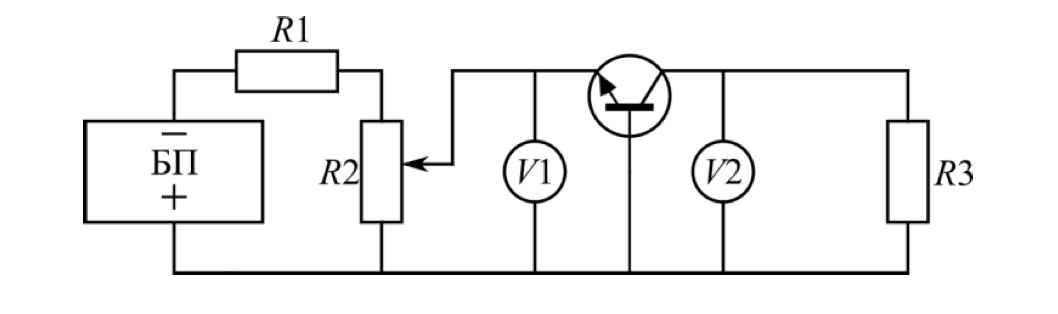
\includegraphics[width=0.6\textwidth]{схема установки7.png} \\
    \end{tabular}
    \caption{Схема экспериментальной установки}
    \label{fig:setup}
\end{figure}


\textbf{Параметры установки:}

Температура в лаборатории: $t = 25 \, ^\circ\text{C}$, $T = 298 \, \text{К}$.

Сопротивление резистора $R_3 = 12,0 \, \text{Ом}$.


\subsection{Обработка результатов измерений}

\subsubsection{Таблицы}
В ходе эксперимента были получены данные, представленные в таблицах ниже.

\begin{table}[H]
    \centering
    \caption{Результаты измерения напряжения и тока}
    \label{tabl:1}
    \begin{tabular}{|c|c|c|c|c|}
        \hline
        № п/п & $U_{\text{эб}}$, В & $U_{\text{кб}}$, В & $I_{\text{к}} = U_{\text{кб}}/R_3$, мА & $\ln I_{\text{к}}$ \\
        \hline
        1  & 0,30 & 0,0026 & 0,0002 & -8,5172 \\
        2  & 0,31 & 0,0039 & 0,0003 & -8,1117 \\
        3  & 0,32 & 0,0075 & 0,0006 & -7,4186 \\
        4  & 0,33 & 0,0121 & 0,0010 & -6,9078 \\
        5  & 0,34 & 0,0195 & 0,0016 & -6,4378 \\
        6  & 0,35 & 0,0287 & 0,0024 & -6,0323 \\
        7  & 0,36 & 0,0391 & 0,0033 & -5,7138 \\
        8  & 0,37 & 0,0563 & 0,0047 & -5,3602 \\
        9  & 0,38 & 0,0756 & 0,0063 & -5,0672 \\
        10 & 0,39 & 0,0900 & 0,0075 & -4,8929 \\
        11 & 0,40 & 0,1204 & 0,0100 & -4,6052 \\
        12 & 0,41 & 0,1481 & 0,0123 & -4,3982 \\
        13 & 0,42 & 0,1838 & 0,0155 & -4,1669 \\
        14 & 0,43 & 0,2065 & 0,0172 & -4,0628 \\
        15 & 0,44 & 0,2299 & 0,0192 & -3,9528 \\
        16 & 0,45 & 0,2623 & 0,0219 & -3,821 \\
        \hline
    \end{tabular}
\end{table}

\subsubsection{ Определение тангенса угла наклона методом парных точек}

Выборка делится на две равные части (по 8 точек). Для каждой пары точек $(x_I, y_I)$ и $(x_{II}, y_{II})$ вычисляется:

\[
a_i = \frac{y_{II} - y_I}{x_{II} - x_I}, \quad \text{где } x = U_{\text{эб}}, \ y = \ln I_{\text{к}}
\]
\begin{table}[H]
\centering
\caption{Вычисление параметров прямой методом парных точек}
\begin{tabular}{|c|c|c|c|c|c|c|c|c|c|}
\hline
№ & $x_I$ & $x_{II}$ & $\Delta x$ & $y_I$ & $y_{II}$ & $\Delta y$ & $a_i$ & $a_i-\bar{a}$ & $(a_i-\bar{a})^2$ \\
\hline
1 & 0,30 & 0,38 & 0,08 & -8,5172 & -5,0672 & 3,4500 & 43,1250 & 12,6061 & 158,91 \\
2 & 0,31 & 0,39 & 0,08 & -8,1117 & -4,8929 & 3,2188 & 40,2350 & 9,7161 & 94,40 \\
3 & 0,32 & 0,40 & 0,08 & -7,4186 & -4,6052 & 2,8134 & 35,1675 & 4,6486 & 21,61 \\
4 & 0,33 & 0,41 & 0,08 & -6,9078 & -4,3982 & 2,5096 & 31,3700 & 0,8511 & 0,72 \\
5 & 0,34 & 0,42 & 0,08 & -6,4378 & -4,1669 & 2,2709 & 28,3863 & -2,1326 & 4,55 \\
6 & 0,35 & 0,43 & 0,08 & -6,0323 & -4,0628 & 1,9695 & 24,6188 & -5,9001 & 34,81 \\
7 & 0,36 & 0,44 & 0,08 & -5,7138 & -3,9528 & 1,7610 & 22,0125 & -8,5064 & 72,36 \\
8 & 0,37 & 0,45 & 0,08 & -5,3602 & -3,8213 & 1,5389 & 19,2363 & -11,2826 & 127,30 \\
\hline
\multicolumn{7}{|c|}{} &\multicolumn{1}{|c|}{$\sum = 244,15$} & \multicolumn{1}{|c|}{} & \multicolumn{1}{|c|}{$\sum = 514,67$} \\
\hline
\end{tabular}
\end{table}

\[
\bar{a} = \frac{244,1514}{8} = 30,5189 \, \text{В}^{-1}
\]
\subsubsection{Оценка погрешности тангенса угла наклона}

Доверительная вероятность $P = 0,95$ означает, что $95\%$ случайных погрешностей не превышают по модулю доверительный интервал $\Delta a$. Для нормального распределения и малого числа измерений ($n = 8$) используется коэффициент Стьюдента $t_{0,95}(7) = 2,365$.

Погрешность вычисляется по формуле:

\[
\Delta a = t_{0,95}(7) \cdot \sqrt{\frac{\sum (a_i - \bar{a})^2}{n(n-1)}}
\]

Подставляя данные из таблицы 2:

\[
\sum (a_i - \bar{a})^2 = 514,67, \quad n = 8
\]

\[
\Delta a = 2,365 \cdot \sqrt{\frac{514,67}{56}}  = 7,17 \; \text{В}^{-1}
\]

Таким образом:

\[
{\tg\alpha = 30,52 \pm 7,17 \; \text{В}^{-1}}
\]

\subsubsection{Вычисление отношения $e/k$}

Согласно формуле (4):
\[
\frac{e}{k} = T \cdot \tg\alpha
\]

При комнатной температуре $T = 296,15$ К получаем:
\[
\frac{e}{k} = 296,15 \cdot 30,5189 = 9037,5 \; \text{К/В}
\]

\subsubsection{Погрешность косвенного измерения}

Формула для расчёта погрешности:

\[
\Delta\left(\frac{e}{k}\right) = \sqrt{\frac{1}{9}\left(\frac{\partial(e/k)}{\partial T} \cdot \Delta T\right)^2 + \frac{1}{9}\left(\frac{\partial(e/k)}{\partial (\tg\alpha)} \cdot \Delta(\tg\alpha)\right)^2}
\]

Подставляем значения:

\[
\Delta\left(\frac{e}{k}\right) = \sqrt{\frac{1}{9}(30,5189 \cdot 0,5)^2 + \frac{1}{9}(296,15 \cdot 7,17)^2}  \approx 707,8 \; \text{К/В}
\]

Окончательный результат:

\[
\frac{e}{k} = (9,04 \pm 0,71) \cdot 10^3 \; \text{К/В} \quad (P = 0,95)
\]

\subsection{Построение графиков}

Для определения отношения заряда электрона \( e \) к постоянной Больцмана \( k \) по формуле \( \frac{e}{k} = T \cdot \tg\alpha \) была построена линейная зависимость \( \ln I_k = f(U_{эб}) \). Согласно уравнению (3), \( \ln I_k = \ln I_0 + \frac{e}{kT} U_{эб} \), где тангенс угла наклона прямой \( \tg\alpha = \frac{e}{kT} \). На график по оси абсцисс откладывались значения напряжения \( U_{эб} \) (в вольтах), а по оси ординат — значения натурального логарифма тока коллектора \( \ln I_k \) (где \( I_k \) выражен в мА). По полученным точкам методом парных точек была проведена аппроксимирующая прямая, также на график были нанесены эксперементальные точки. На основании построенного графика (рис. 1) был определён тангенс угла наклона \( \tg\alpha \), который составил \( 30,5189 \, \text{В}^{-1} \).

\begin{figure}[H]
\centering
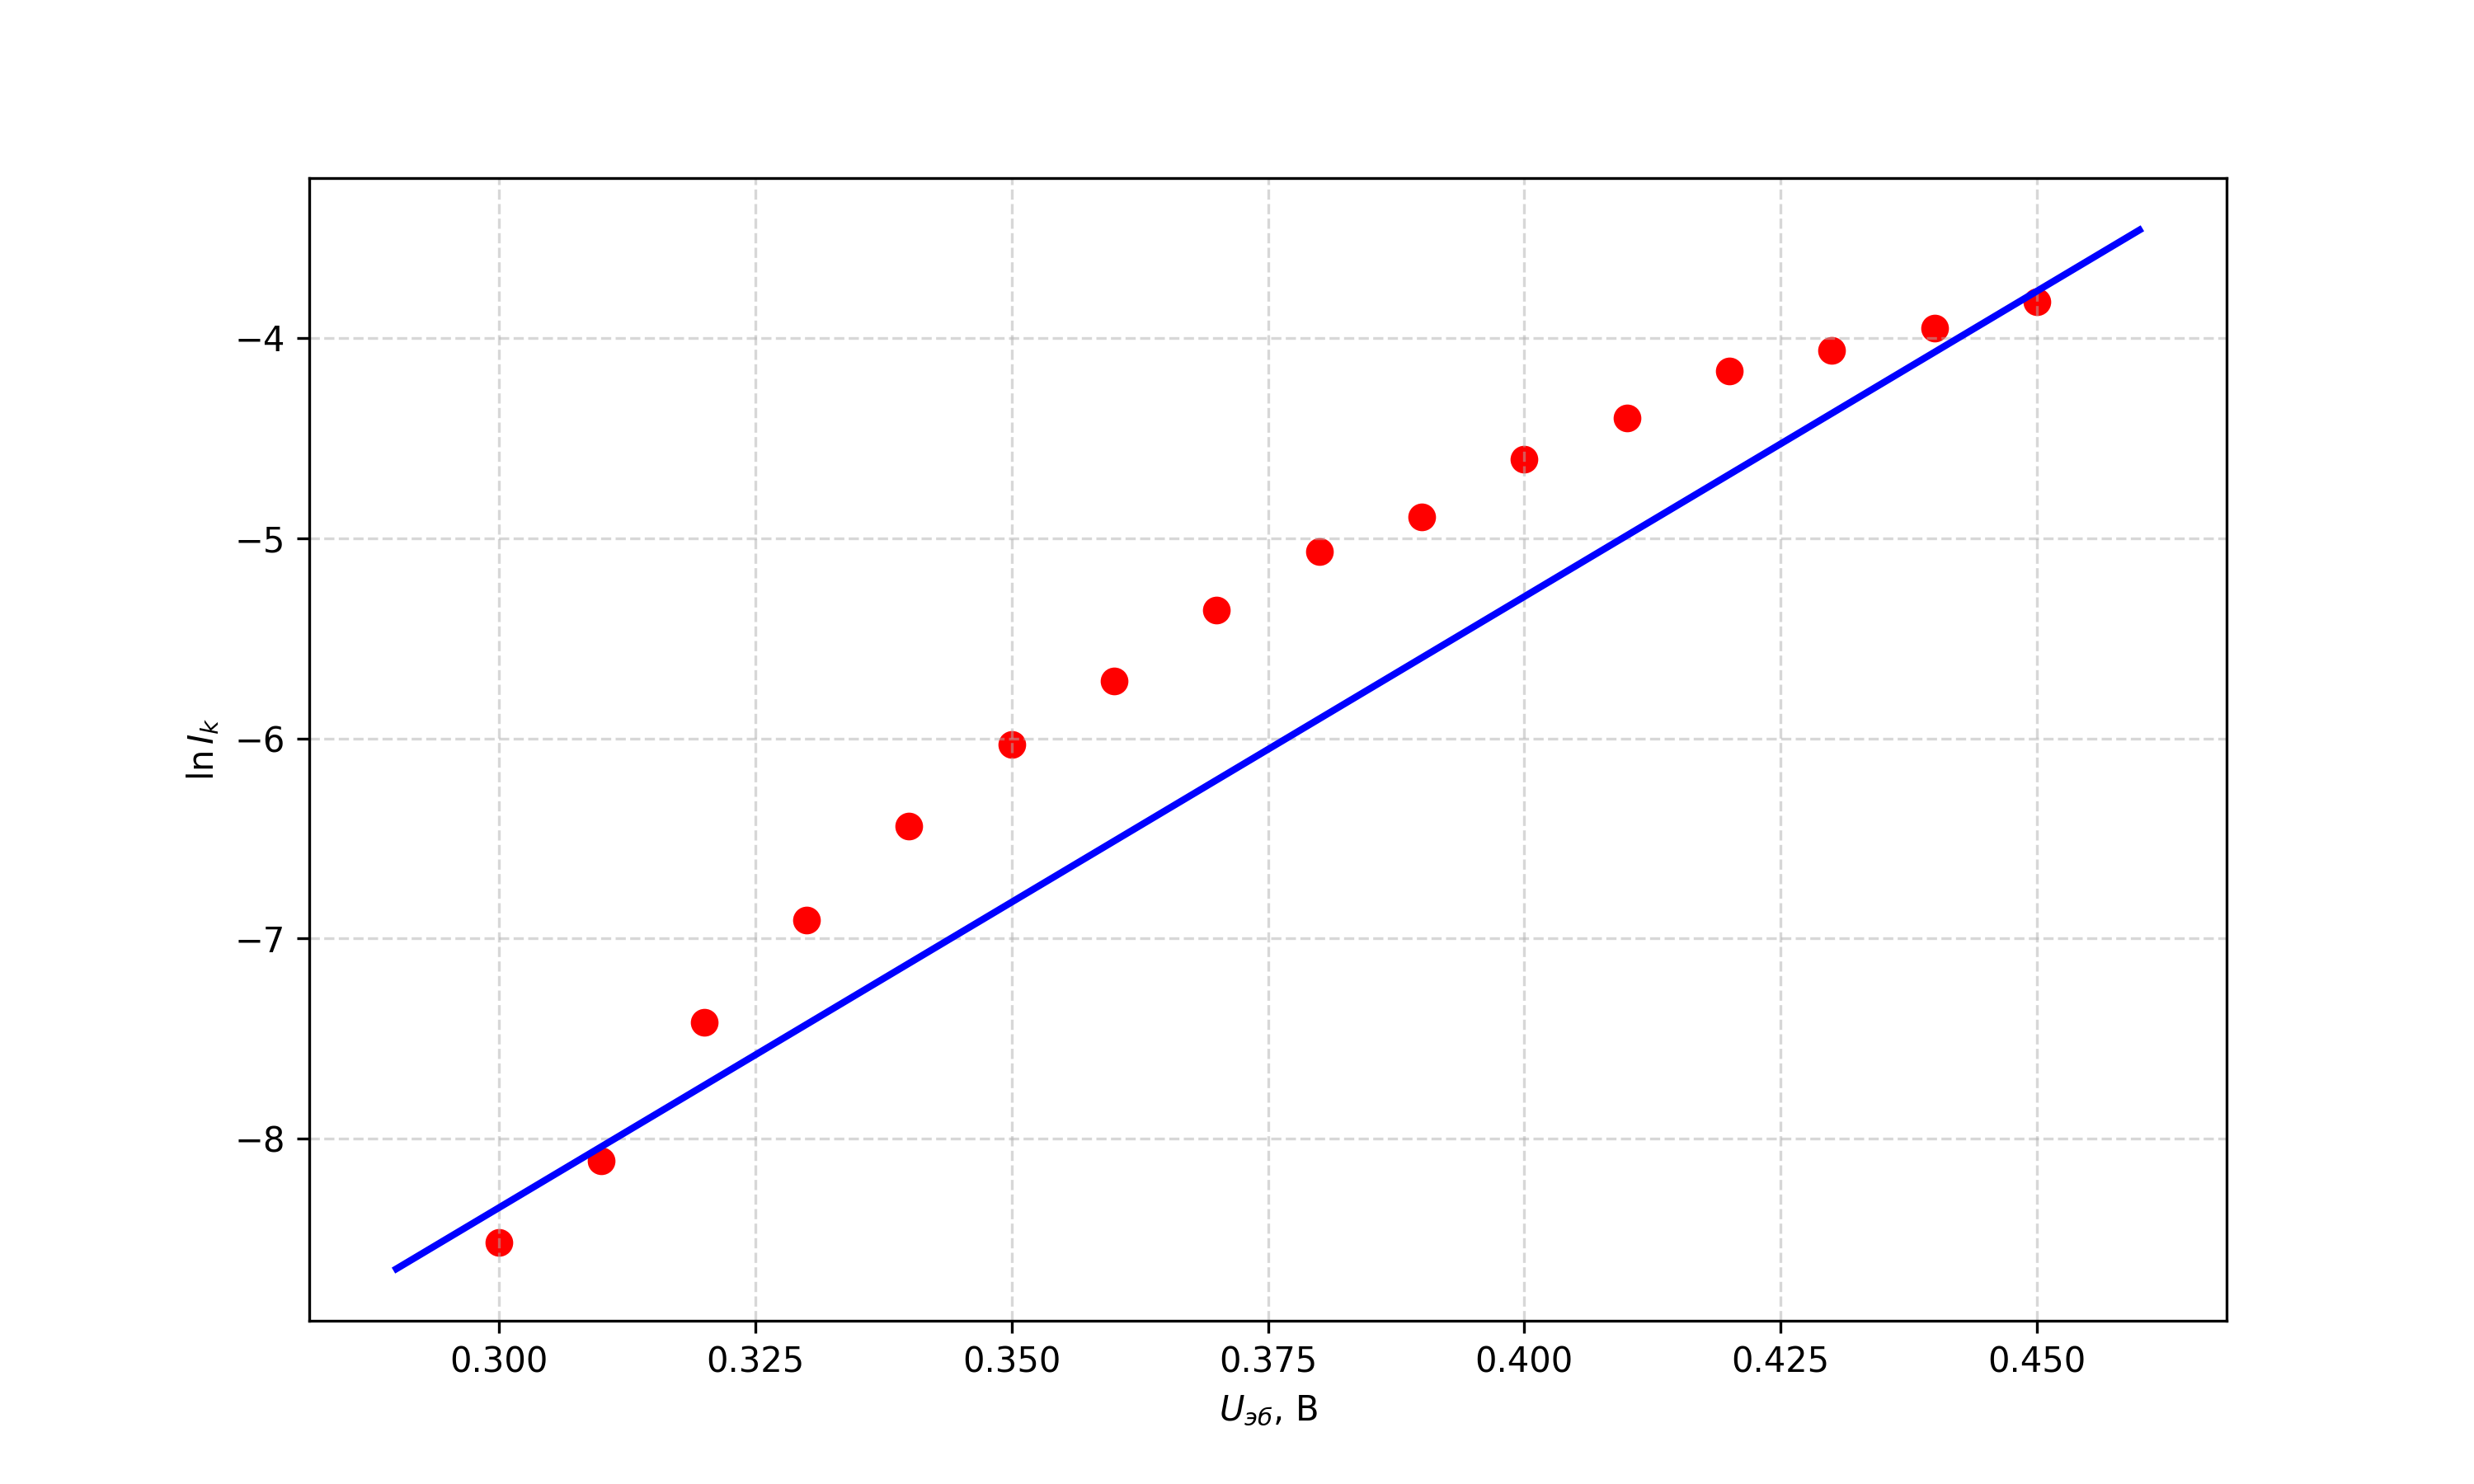
\includegraphics[width=0.8\textwidth]{graph1.png}
\caption{Зависимость \( \ln I_k = f(U_{эб}) \) для выборки 1}
\end{figure}

Далее по формуле \( \frac{e}{k} = T \cdot \tg\alpha \) было вычислено искомое отношение. При комнатной температуре \( T = 296,15 \, \text{К} \) получено значение \( \frac{e}{k} = 9037,5 \, \text{К/В} \).

Кроме того, была построена экспоненциальная зависимость \( I_k = I_0 e^{\frac{e}{kT} U_{эб}} \) (рис. 2). На этом графике по оси абсцисс отложено напряжение \( U_{эб} \) (В), а по оси ординат — ток коллектора \( I_k \) (мА). Аппроксимирующая кривая построена на основе найденных параметров \( \tg\alpha \) и \( \ln I_0 \). Значение тока насыщения, полученное из графика, составило \( I_0 = \exp(\ln I_0) \approx 2,5 \cdot 10^{-8} \, \text{мА} \).

\begin{figure}[H]
\centering
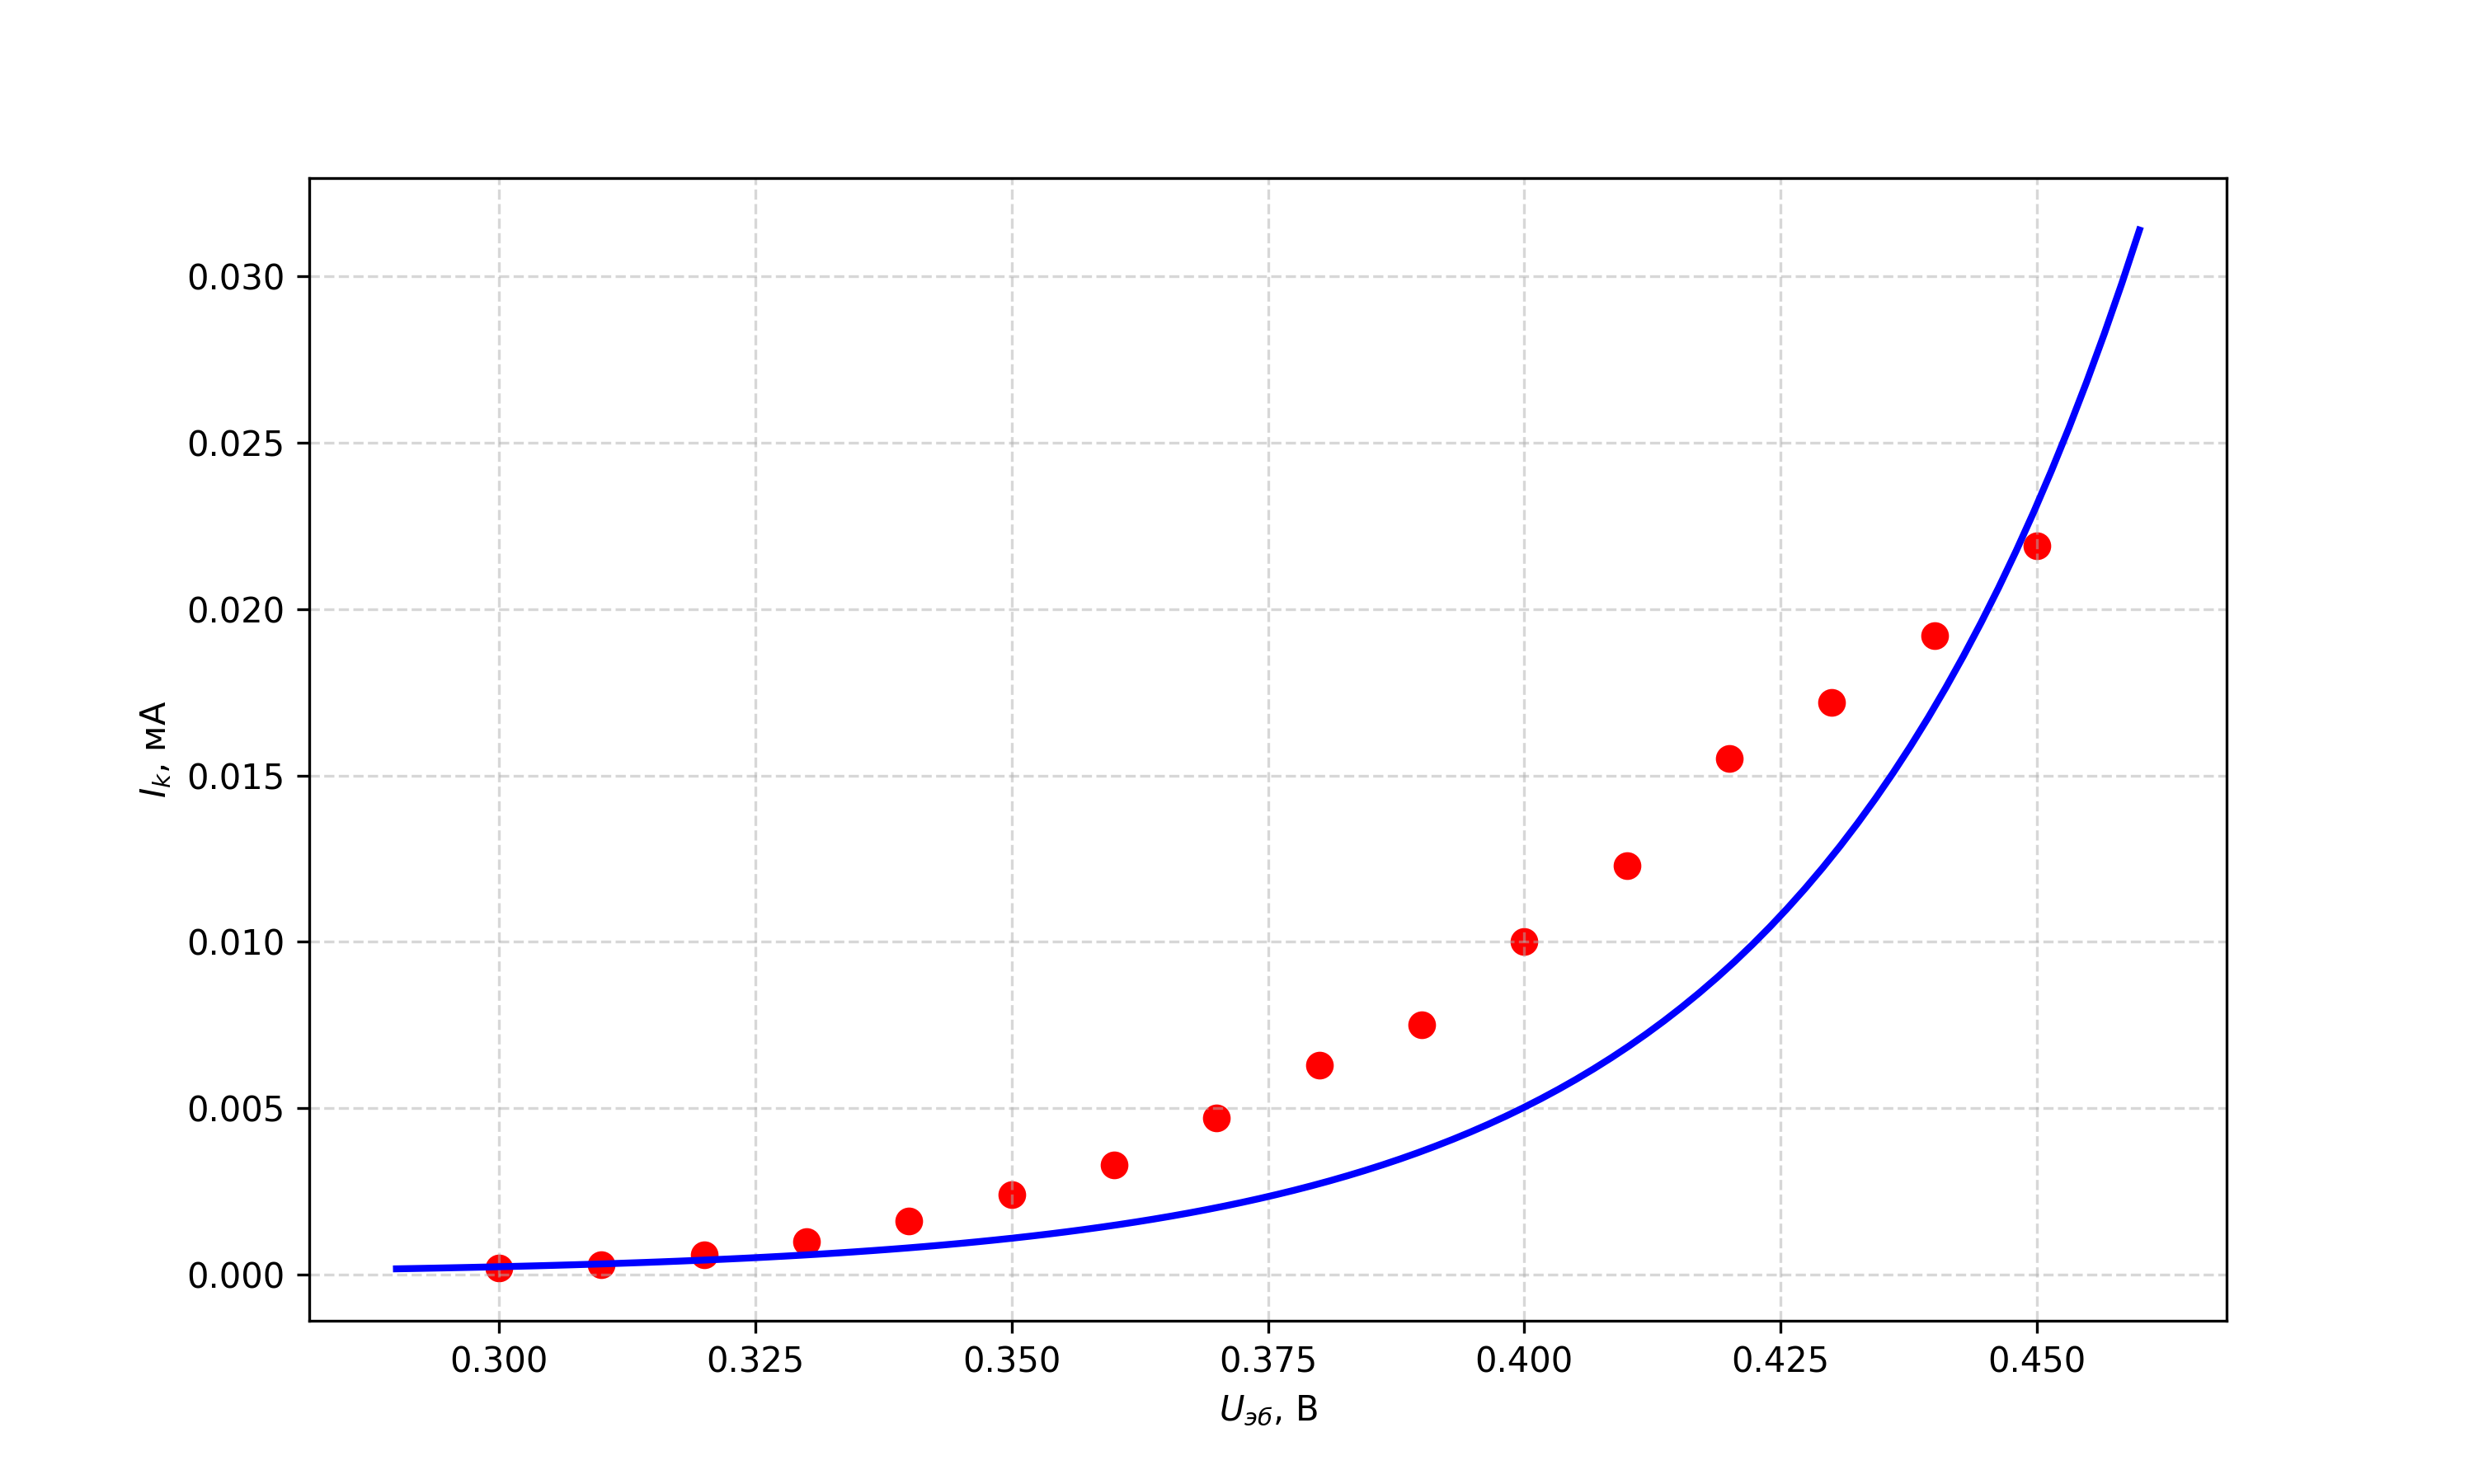
\includegraphics[width=0.8\textwidth]{graph2.png}
\caption{Зависимость \( I_k = f(U_{эб}) \) для выборки 1}
\end{figure}

\section{Выводы}

В ходе эксперимента была измерена зависимость тока короткого замыкания коллектора биполярного транзистора от напряжения между эмиттером и базой. Построена зависимость $\ln I_{\text{к}} = f(U_{\text{эб}})$, подтверждающая линейный характер в соответствии с уравнением (3). Методом парных точек определён тангенс угла наклона прямой и рассчитано отношение заряда электрона к постоянной Больцмана $\frac{e}{k}$.

Полученные значения составляют:

\[
\tg\alpha = 30,52 \pm 7,17 \; \text{В}^{-1} \quad (P = 0,95)
\]

\[
\frac{e}{k} = 9,09 \times 10^3 \, \text{Кл/Дж}
\]

В ходе работы экспериментально подтверждена экспоненциальная зависимость тока коллектора биполярного транзистора от напряжения эмиттер-база: \( I_k = I_0 e^{\frac{eU_{эб}}{kT}} \). Построены графики \( \ln I_k = f(U_{эб}) \) и \( I_k = f(U_{эб}) \), по которым методом парных точек определён тангенс угла наклона \( \tg\alpha = 30,5189 \, \text{В}^{-1} \).

При комнатной температуре \( T = 296,15 \, \text{К} \) вычислено отношение заряда электрона к постоянной Больцмана:

\[
\frac{e}{k} = T \cdot \tg\alpha = 9037,5 \, \text{К/В}.
\]

Полученное значение отличается от теоретического \( 11604 \, \text{К/В} \) на \( 2567\, \text{К/В} \). Основная причина расхождения — малые значения \( U_{эб} \) (0,30 – 0,45 В), при которых пренебрежение единицей в формуле \( I_k = I_0(e^{\frac{eU}{kT}} - 1) \) даёт значительную погрешность. Для повышения точности измерения следует проводить при более больших значениях.

\clearpage
\appendix


\end{document}
